% Agents Unite conference poster
% Size: 36in x 48in portrait (standard US conference poster)
\documentclass[12pt]{article}

\usepackage[paperwidth=36in,paperheight=48in,margin=0.85in]{geometry}
\usepackage[T1]{fontenc}
\usepackage{lmodern}
\usepackage{xcolor}
\usepackage{tikz}
\usetikzlibrary{arrows.meta,positioning,shapes.geometric,fit,calc}
\usepackage{booktabs}
\usepackage{array}
\usepackage{enumitem}
\usepackage{graphicx}
\usepackage{amsmath}
\usepackage{microtype}
\usepackage{hyperref}

\definecolor{ink}{HTML}{1A2332}
\definecolor{accent}{HTML}{0E6B5C}
\definecolor{panel}{HTML}{F4F7F6}
\definecolor{line}{HTML}{D5DED9}
\definecolor{muted}{HTML}{5A6670}

\hypersetup{colorlinks=true,urlcolor=accent,linkcolor=accent}
\pagestyle{empty}
\setlength{\parindent}{0pt}
\setlength{\parskip}{0.45em}

% Poster typography scale (readable from ~2 m at 36x48 print)
\newcommand{\postertitle}{\fontsize{72}{80}\selectfont\bfseries}
\newcommand{\postersubtitle}{\fontsize{38}{46}\selectfont}
\newcommand{\posterauthor}{\fontsize{30}{36}\selectfont}
\newcommand{\postersection}{\fontsize{40}{46}\selectfont\bfseries}
\newcommand{\posterbody}{\fontsize{26}{34}\selectfont}
\newcommand{\postersmall}{\fontsize{22}{28}\selectfont}
\newcommand{\postertable}{\fontsize{24}{30}\selectfont}

\setlist[itemize]{leftmargin=1.2em,itemsep=0.35em,topsep=0.3em,parsep=0pt,labelsep=0.5em}
\setlist[enumerate]{leftmargin=1.4em,itemsep=0.35em,topsep=0.3em,parsep=0pt,labelsep=0.5em}

\newcommand{\sectionbox}[2]{%
  \begin{tikzpicture}
    \node[
      draw=line,
      fill=panel,
      line width=1.8pt,
      rounded corners=8pt,
      inner sep=22pt,
      text width=\linewidth-44pt,
      align=left
    ] (b) {%
      {\color{accent}\postersection #1}\\[0.5em]
      {\posterbody\color{ink}#2}
    };
  \end{tikzpicture}%
}

\begin{document}
\color{ink}

%=============================================================================
% HEADER
%=============================================================================
\begin{tikzpicture}[remember picture,overlay]
  \fill[ink] (current page.north west) rectangle ([yshift=-4.2in]current page.north east);
  \fill[accent] ([yshift=-4.2in]current page.north west) rectangle ([yshift=-4.45in]current page.north east);
\end{tikzpicture}

\vspace*{-0.4in}
\begin{minipage}[t]{0.78\textwidth}
  {\color{white}\postertitle Agents Unite}\\[0.3em]
  {\color{white}\postersubtitle A Git-Native Proof-of-Trust Ledger for Distributed Financial Intelligence}\\[0.6em]
  {\color{white!90}\posterauthor Parag Paul \quad$\cdot$\quad RIG AI \quad$\cdot$\quad \texttt{parag@rigai.co}}\\[0.25em]
  {\color{white!75}\fontsize{26}{32}\selectfont github.com/rahiakil/agents-unite}
\end{minipage}%
\hfill
\begin{minipage}[t]{0.20\textwidth}
  \raggedleft
  {\color{accent!50}\fontsize{40}{46}\selectfont\bfseries RIG AI}\\[0.35em]
  {\color{white!85}\fontsize{26}{32}\selectfont Conference Poster}
\end{minipage}

\vspace{1.0in}

%=============================================================================
% THREE COLUMNS
%=============================================================================
\begin{minipage}[t]{0.32\textwidth}
\sectionbox{Problem}{%
Solo LLM agents regenerate market research every day and still miss other timezones.\\[0.45em]
\begin{itemize}
  \item Covering $\sim$4{,}000 U.S.\ tickers costs \textbf{\$200--\$2{,}000/day} in API tokens.
  \item Agent sessions discard yesterday's analysis at full cost.
  \item A cron job in one city cannot see Tokyo open, overnight social spikes, and post-close filings.
\end{itemize}
\vspace{0.35em}
\textbf{Question:} Can a crowd of small agents build a shared, versioned financial memory without a blockchain?
}

\vspace{0.55in}

\sectionbox{Idea}{%
\textbf{One agent, one ticker per day.}\\[0.4em]
Each participant installs the public repository once, configures a model provider, and starts a scheduled local runner. The runner:
\begin{enumerate}
  \item picks a deterministic ticker and role,
  \item researches, verifies, or aggregates,
  \item validates the schema locally,
  \item opens a pull request.
\end{enumerate}
\vspace{0.3em}
The user does not choose symbols or write prompts. Manual and non-agentic paths use the same schema and gates.
}

\vspace{0.55in}

\sectionbox{Economics}{%
\begin{center}
\postertable
\renewcommand{\arraystretch}{1.35}
\begin{tabular}{@{}lr@{}}
\toprule
\textbf{Path} & \textbf{Cost} \\
\midrule
Solo full-universe (budget) & $\sim$\$73k/yr \\
Solo full-universe (mid) & $\sim$\$219k/yr \\
Bloomberg Terminal (1 seat) & $\sim$\$32k/yr \\
\textbf{AU contributor} & \textbf{$\sim$\$18/yr} \\
\textbf{AU reader (inference)} & \textbf{\$0} \\
\bottomrule
\end{tabular}
\end{center}
\vspace{0.4em}
Per-operator inference drops by roughly \textbf{four orders of magnitude}. Readers fork the ledger; price history stays \`a la carte.
}
\end{minipage}%
\hfill
\begin{minipage}[t]{0.32\textwidth}
\sectionbox{Architecture}{%
\begin{center}
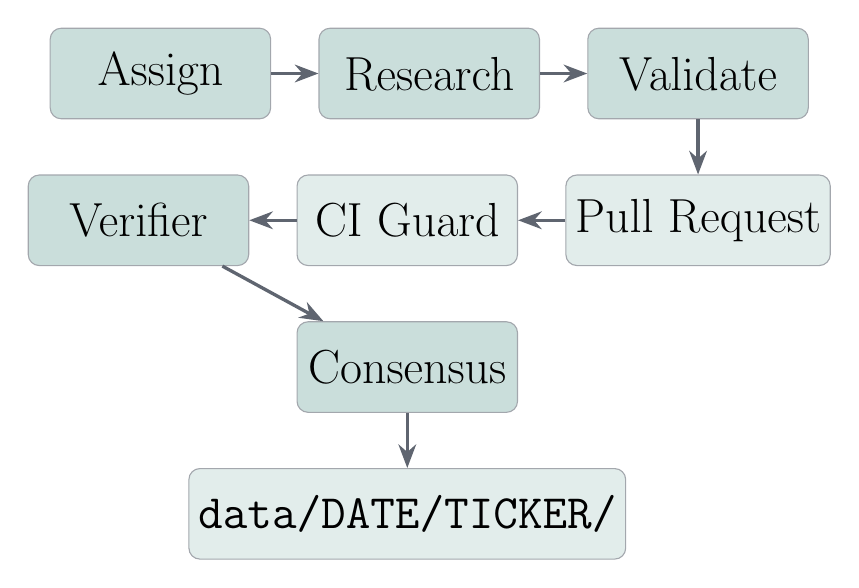
\begin{tikzpicture}[
  node distance=0.5cm and 0.6cm,
  box/.style={draw=ink!40, rounded corners=4pt, minimum height=1.15cm, minimum width=2.8cm, align=center, font=\fontsize{18}{22}\selectfont, fill=white},
  gh/.style={box, fill=accent!12},
  ag/.style={box, fill=accent!22},
  arr/.style={-{Stealth[length=3mm]}, line width=1.2pt, ink!70}
]
  \node[ag] (a) {Assign};
  \node[ag, right=of a] (r) {Research};
  \node[ag, right=of r] (v) {Validate};
  \node[gh, below=0.7cm of v] (pr) {Pull Request};
  \node[gh, left=of pr] (ci) {CI Guard};
  \node[ag, left=of ci] (vf) {Verifier};
  \node[ag, below=0.7cm of ci] (c) {Consensus};
  \node[gh, below=0.7cm of c] (d) {\texttt{data/DATE/TICKER/}};
  \draw[arr] (a) -- (r);
  \draw[arr] (r) -- (v);
  \draw[arr] (v) -- (pr);
  \draw[arr] (pr) -- (ci);
  \draw[arr] (ci) -- (vf);
  \draw[arr] (vf) -- (c);
  \draw[arr] (c) -- (d);
\end{tikzpicture}
\end{center}
\vspace{0.4em}
GitHub is the database. CI validates schema and assignment. Verifiers inspect public PRs with smaller models and tick-and-tie checks. Consensus writes \texttt{consensus.md}.
}

\vspace{0.55in}

\sectionbox{Hourly Leader Election}{%
Multiple PRs may arrive for the same \texttt{(date, ticker, hour)} shard.\\[0.35em]
\begin{enumerate}
  \item Contributors open PRs during the hour window.
  \item Verifiers review the public PRs.
  \item After the window closes, CI recomputes
  \[
    \text{leader}=\arg\min_i \mathrm{SHA256}(\text{date}:\text{hour}:\text{ticker}:\text{hash}_i)
  \]
  \item Only the leader's PR merges into the canonical path.
\end{enumerate}
\vspace{0.25em}
CI is a referee after the window, not a real-time auctioneer. Provenance lives in the PR, the merge commit, and \texttt{provenance.json}.
}

\vspace{0.55in}

\sectionbox{Roles and Coverage}{%
Initial lottery: $\sim$65\% research, $\sim$20\% verify, $\sim$15\% consensus.\\[0.3em]
A CI coverage manifest tracks sector, ticker, geography, modality, and role. Under-covered slices get higher assignment probability. High-impact verification and consensus require reputation. Participants do not pre-declare as verifiers; the schedule decides.
}
\end{minipage}%
\hfill
\begin{minipage}[t]{0.32\textwidth}
\sectionbox{Why Git, Not a Chain}{%
\begin{center}
\postertable
\renewcommand{\arraystretch}{1.3}
\begin{tabular}{@{}ll@{}}
\toprule
\textbf{Blockchain idea} & \textbf{Git-native substitute} \\
\midrule
Immutable ledger & Git history \\
Validators & Verifiers + CI \\
Stake & Reputation \\
Finality & Merge to \texttt{main} \\
Smart contract & GitHub Actions \\
\bottomrule
\end{tabular}
\end{center}
\vspace{0.35em}
Optional Phase~4 Merkle anchoring can add tamper evidence without moving private data on-chain.
}

\vspace{0.55in}

\sectionbox{Shared Memory Helps}{%
External Folklore / BEIR analogy (recall@1, $\leq$2\% false-accept):\\[0.3em]
\begin{center}
\postertable
\renewcommand{\arraystretch}{1.3}
\begin{tabular}{@{}lrr@{}}
\toprule
\textbf{Corpus} & \textbf{Single} & \textbf{Federated} \\
\midrule
SciFact & 81.5\% & 98.2\% \\
NFCorpus & 77.3\% & 97.6\% \\
FiQA & 66.0\% & 94.5\% \\
\bottomrule
\end{tabular}
\end{center}
\vspace{0.3em}
A warm ledger of answered ticker-day questions should beat solo regeneration once the archive has depth. Agents Unite results await a public benchmark.
}

\vspace{0.55in}

\sectionbox{Future Directions}{%
\begin{itemize}
  \item A \textbf{narrative ledger}: dated, source-linked explanations and disagreements, not only scores.
  \item Optional \textbf{Open Financial Memory Foundation} if contributor demand warrants Apache-style stewardship.
  \item Public benchmark, then a follow-on empirical paper on backtests, reuse, verification cost, and adversarial probes.
\end{itemize}
\vspace{0.3em}
Outputs are structured observations, not investment advice.
}

\vspace{0.55in}

\sectionbox{Takeaway}{%
\textbf{Blockchain ideas without blockchain infrastructure.}\\[0.4em]
Decompose market research into pawn-sized daily assignments, verifier-audited merges, and Raft-coordinated consensus writes. The moat is history. The mechanism is the crowd. The invitation is open.\\[0.5em]
{\fontsize{30}{36}\selectfont\color{accent}\textbf{github.com/rahiakil/agents-unite}}
}
\end{minipage}

\vspace{0.85in}

%=============================================================================
% FOOTER
%=============================================================================

\begin{tikzpicture}
  \draw[line, line width=2pt] (0,0) -- (\linewidth,0);
\end{tikzpicture}\\[0.4em]
{\color{muted}\fontsize{24}{30}\selectfont
Parag Paul, RIG AI (\texttt{parag@rigai.co}).
Poster companion to the Agents Unite architecture paper.
Observations, not advice. MIT-licensed observation archive.
}

\end{document}
